\begin{figure*}[t!]
\vspace*{-2ex}
\centering

%\begin{tabular}{lll}
%\begin{tabular}{c}
%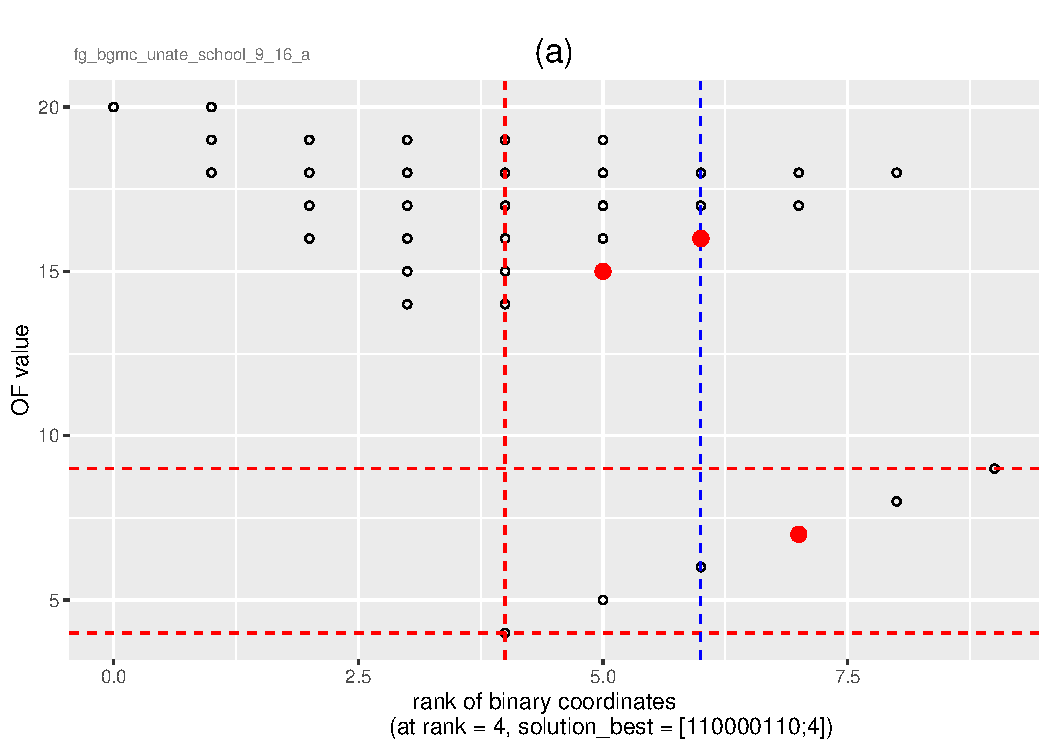
\includegraphics[width=0.50\textwidth]{../_Figures/fg_bgmc/fg_bgmc_unate_school_9_16_a}
%\end{tabular}
%&
%\begin{tabular}{c}
%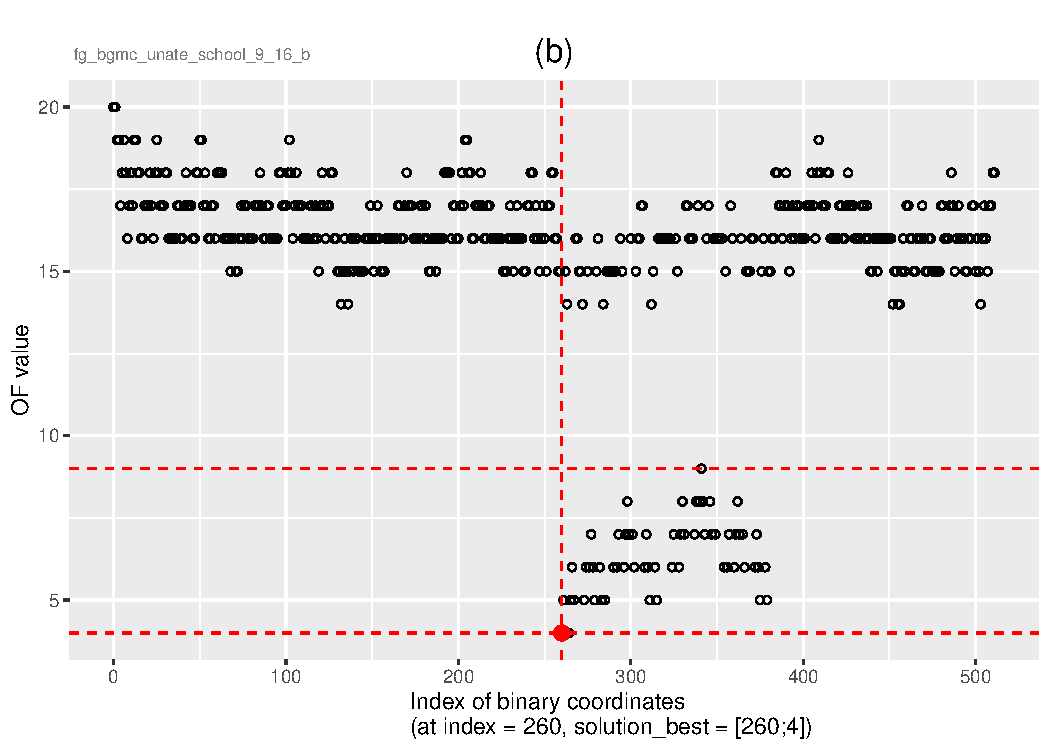
\includegraphics[width=0.50\textwidth]{../_Figures/fg_bgmc/fg_bgmc_unate_school_9_16_b}
%\end{tabular}
%\end{tabular} 

%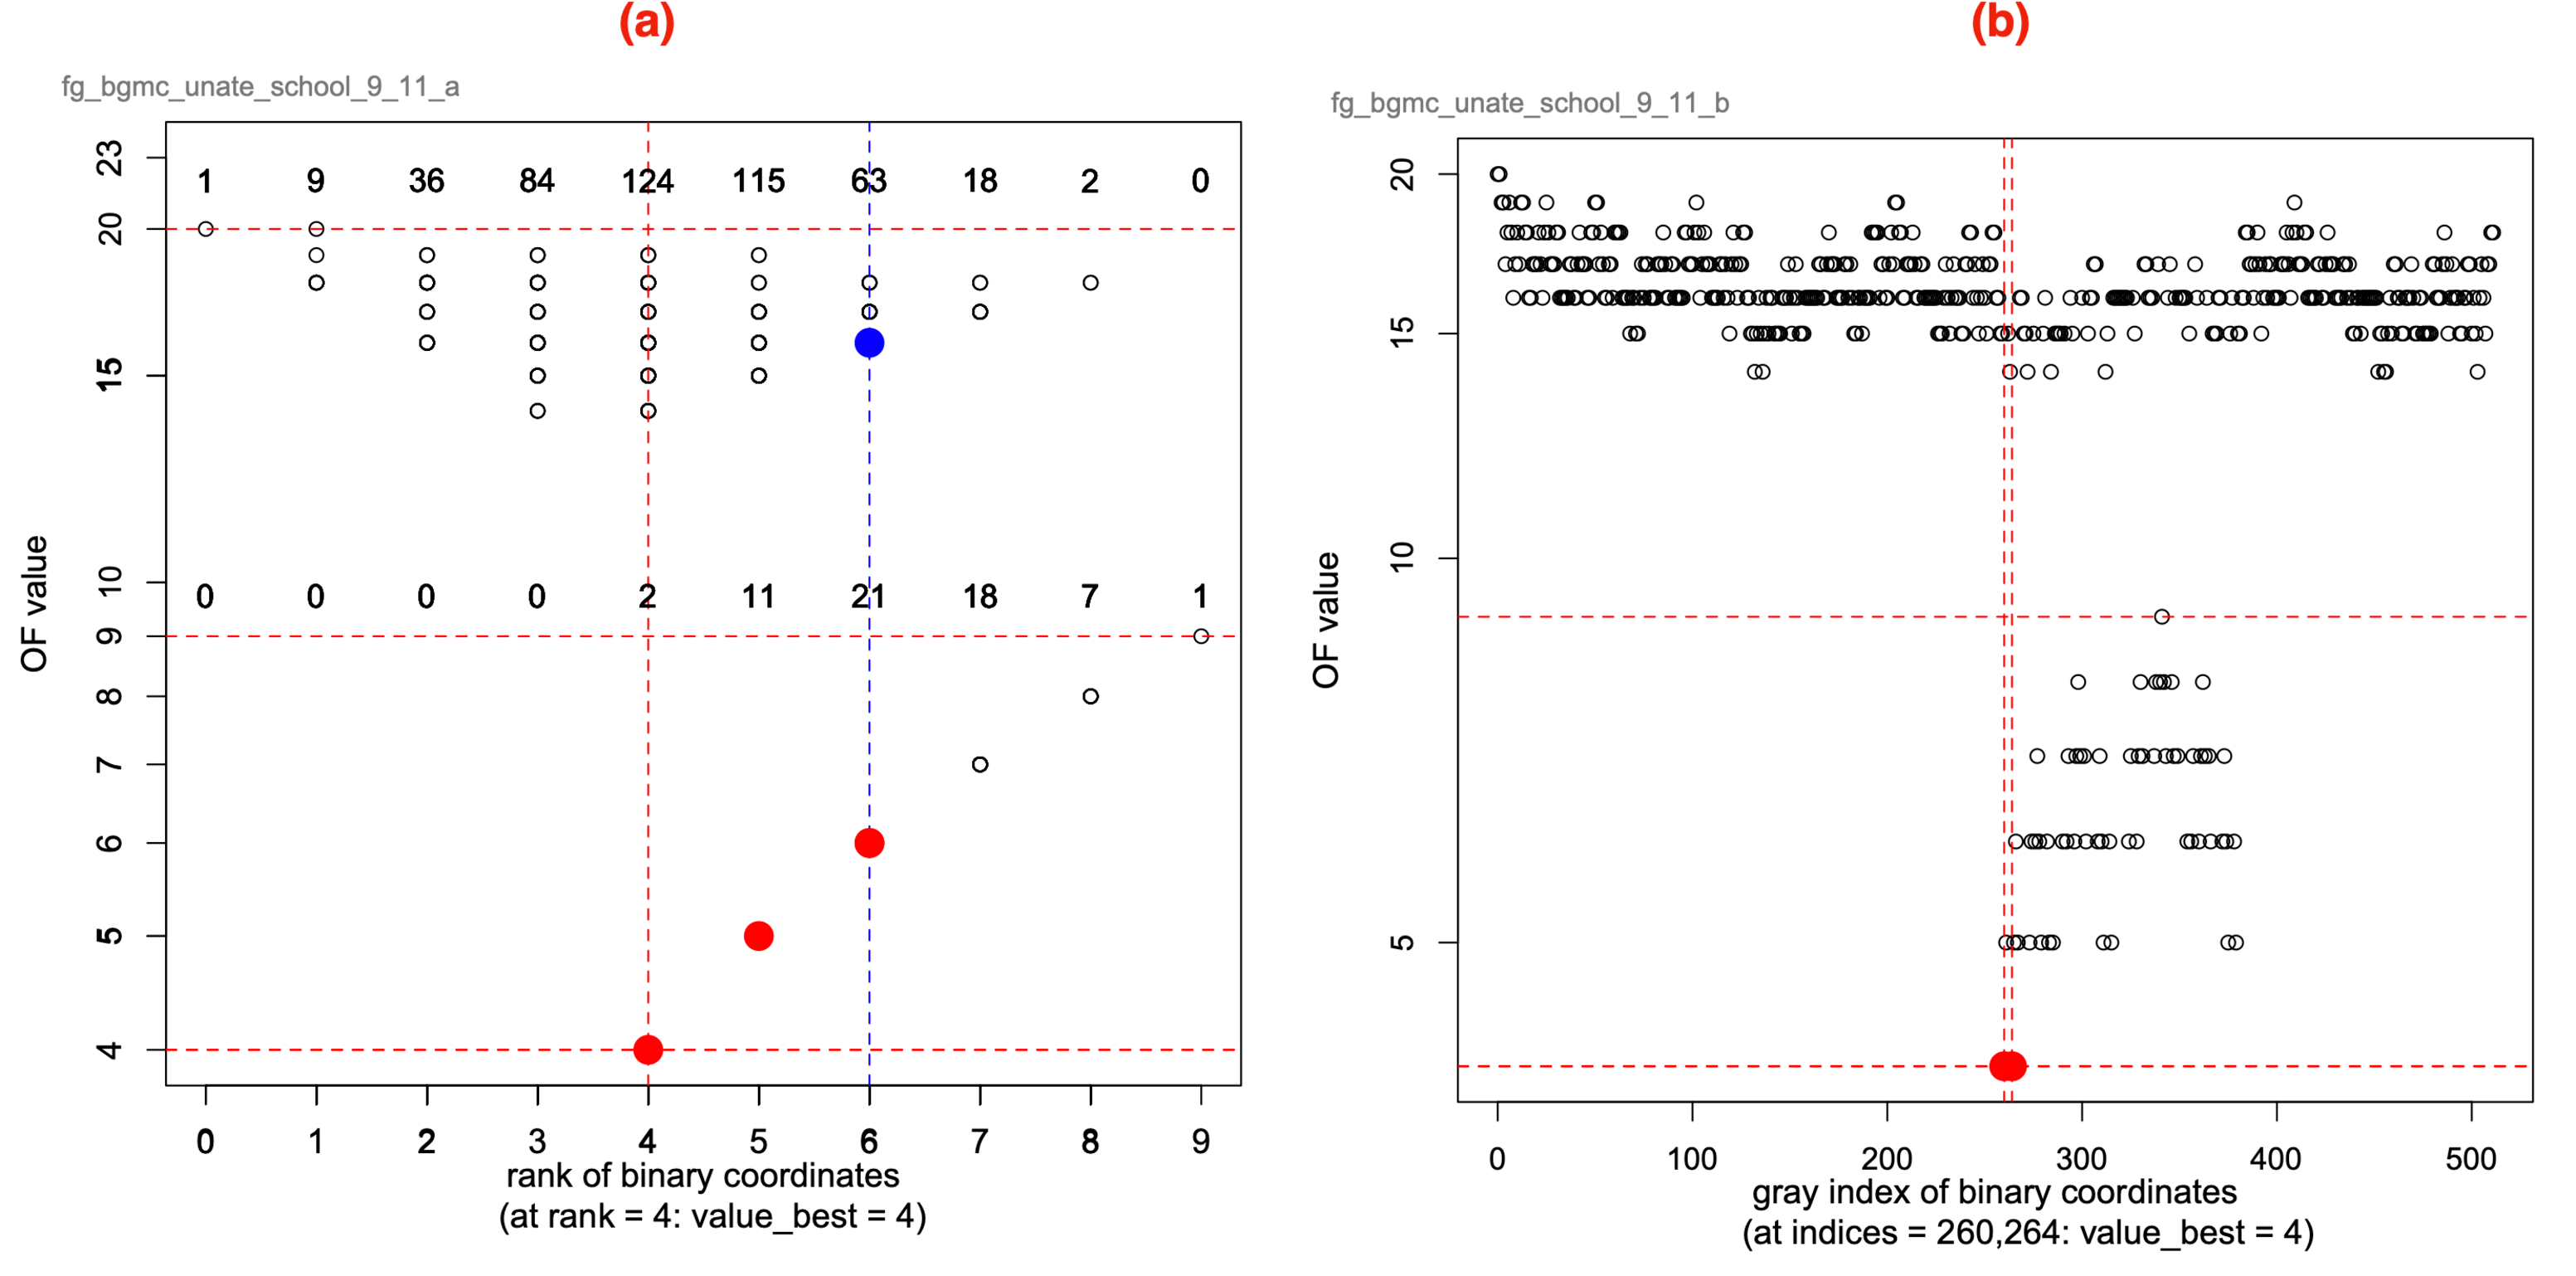
\includegraphics[width=1.01\textwidth]{../_Figures/fg_bgmc/fg_bgmc_unate_school_9_11_ab}

\begin{tabular}{ll}


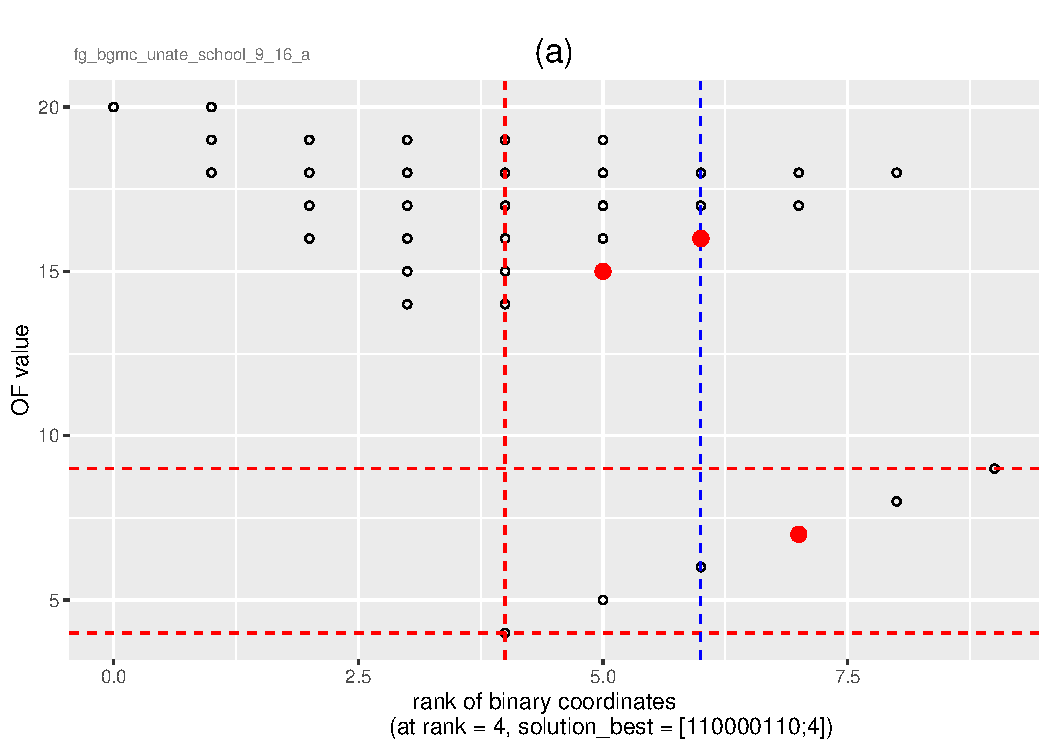
\includegraphics[width=0.49\textwidth]{_Figures/fg_bgmc_unate_school_9_11_a}


&

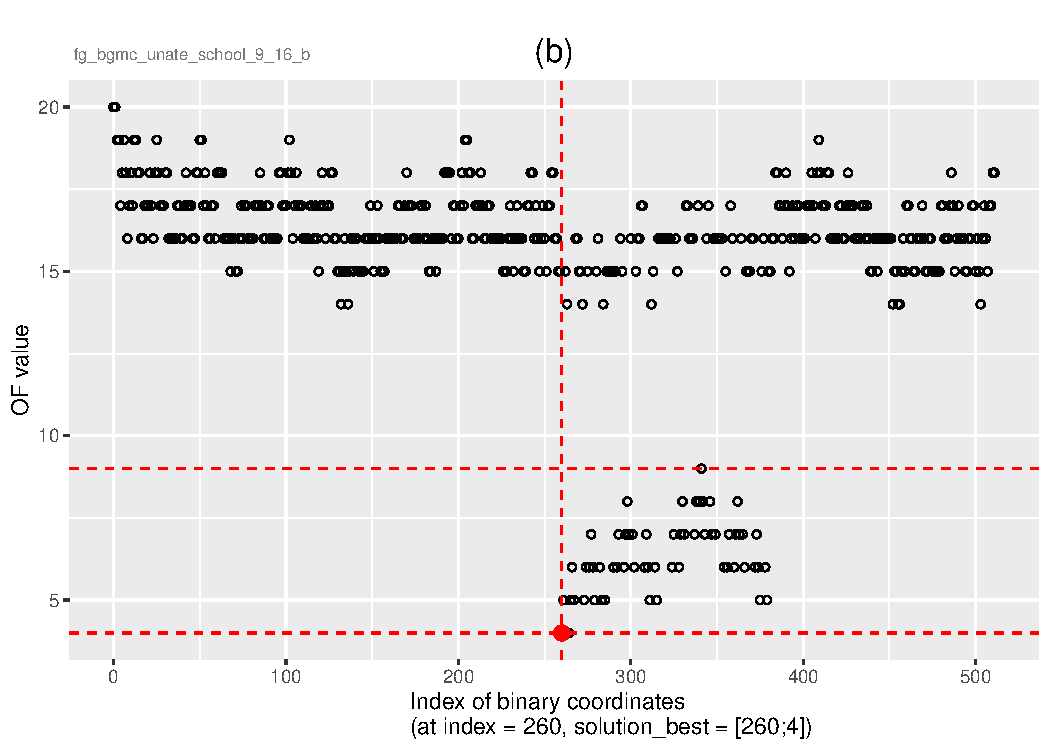
\includegraphics[width=0.49\textwidth]{_Figures/fg_bgmc_unate_school_9_11_b}

\end{tabular}


\caption{
There is no substitute for exhaustive enumeration if we are to learn all we can about
the nature of a combinatorial optimization problem. Here we illustrate additional views
of the unit-weighted unate set cover problem introduced in 
Figure~\ref{fg_bgmc_matching_cover}. 
In (a), we depict values of the {\it objective function} (OF) as a function of
the {\it rank} of binary coordinates.
The labels at y-axis = 22 represent the number of coordinates  that are not 
feasible solutions for this instance.
The labels at y-axis = 9.5 represent the number of coordinates  that are  
feasible solutions for this instance.
In (b), we depict values of the OF as a function of
binary coordinates indexed in {\it gray order}: the first coordinate is $000000000$,
the last coordinate is $100000000$.
All points at y-axis positions $<=$ 9 represent  feasible solutions for this instance.
\\[0.85ex]
\hspace*{2.5ex}Both (a) and (b) suggest a number of heuristics to search for the minimum OF value
in significantly less OF evaluations when compared to $2^n = 512$.
A few simple heuristics are discussed in the text.
}
\label{fg_bgmc_unate_school_9_11}
\end{figure*}
